% Chapter Experiment

\chapter{Experimental Setup at the IP2I cryogenic facility} % Main chapter title

\label{ChapterExperiment} % Change X to a consecutive number; for referencing this chapter elsewhere, use \ref{ChapterX}

%----------------------------------------------------------------------------------------
%	BEGING CHAPTER
%----------------------------------------------------------------------------------------

This chapter describes the IP2I Cyostat Facility in which the cryogenic germanium detectors presented in this work were operated. It explains how cryogenic conditions are obtained, presents the cryogenic germanium detectors and their principle of operation.

\section{The IP2I cryogenic facility}
\label{sec:IP2I-cryostat-facility} 

% Intro
The particles detectors studies in this work are cryogenic germanium bolometers. The term "cryogenic" indicates that these detectors are operated at cryogenic temperatures below $\SI{1}{\kelvin} = \SI{-272,15}{\celsius}$. In order to reach such temperatures, the detectors are placed inside of a cryostat.

The experimental results discussed in this work were obtained by running germanium detectors in the the dry dilution cryostat of the \textit{Institut de Physique des 2 Infinis de Lyon} (IP2I). The IP2I cryogenic facility is located in the basement of the IP2I Haefely building (see figure \ref{fig:haefely-building}). With an almost negligible overburden roughly estimated to be about \SI{1.5}{m.w.e}, the cryogenic detectors are operated in an above-ground or surface experiment as opposed to the underground operation of the EDELWEISS detectors at the LSM.

% Radioactive shielding
In order to reduced the environmental gamma background, the cryostat is surrounded by a \SI{10}{\cm} thick cylindrical lead shield covering a solid angle of $\sim \SI{70}{\percent}$ of $4\pi$ around the detector. A reduction of about a factor of 10 is estimated on the triggering rate of our detectors with this lead shield.
There is no lead shield inside the cryostat. The materials used for the cryostat construction were not selected for low radioactivity, with the exception of the replacement of the standard glass fiber rods used by Cryoconcept by stainless steel ones, shown to have much less radioactive contamination. 
While the radioactive background is high as a consequence of the above-ground operation, it is very similar to what is expected from the ILL site for the \Ricochet{} experiment. The neutron and gamma components of this background are characterized down to \SI{1}{\kilo\eV} in the Chapter \ref{ChapterNeutron}.

\begin{figure}
\centering
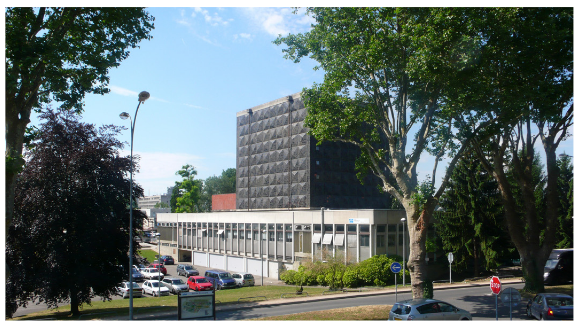
\includegraphics[width=\textwidth,angle=0]{Figures/Experiment/haefely_building.png}
\caption{Photo of the IP2I Haefely building. The cryogenic facility is located in the basement, at the same height as the parking lot.}
\label{fig:haefely-building}
\end{figure}

The total surface area of the facility is about a \SI{100}{\m^2} and encompasses the main cryogenic lab (\SI{80}{\m^2}), a technical room for pumps and gas handling system (\SI{6}{\m^2}), an ISO-5 clean room for detector mounting (\SI{9}{\m^2}), and a room hosting a chemical bench also related to detector fabrication (\SI{5}{\m^2}). A photo of the cryogenic laboratory is displayed in figure \ref{fig:cryolab} with the open cryostat in the corner of the room next to the lead shielding of the left and the acquisition electronics and computers on the right.

\begin{figure}
\begin{center}
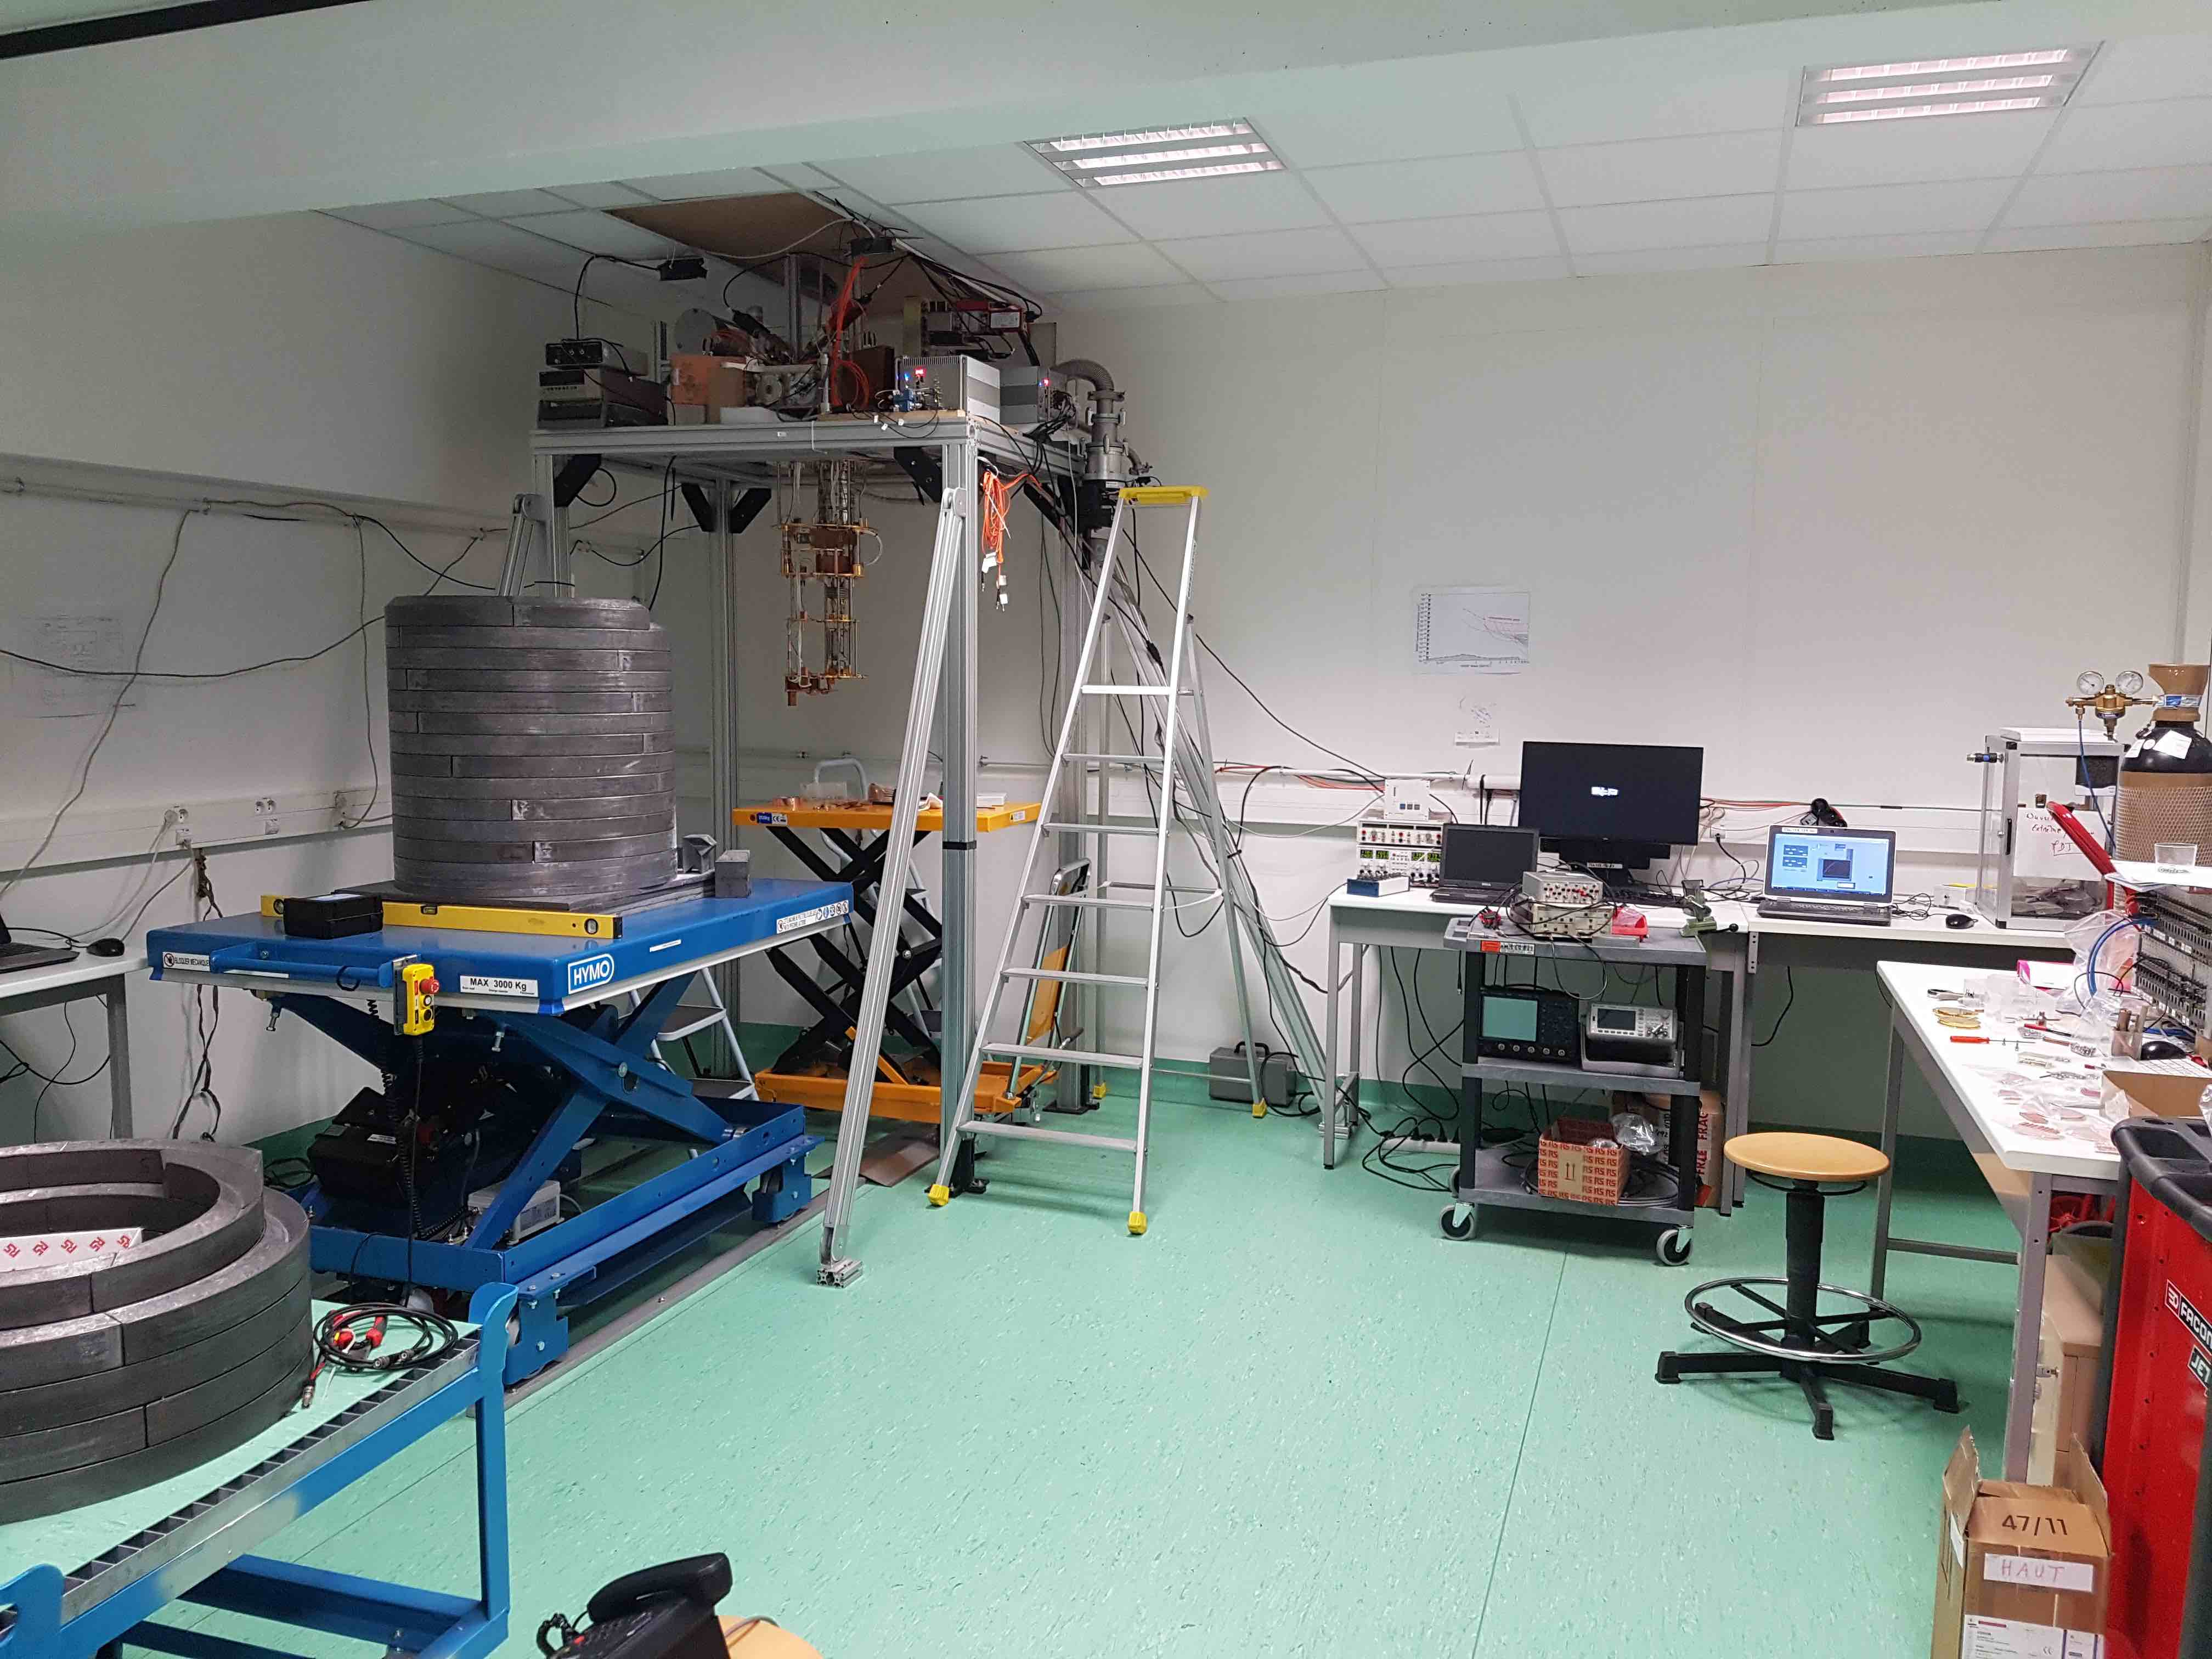
\includegraphics[width=\textwidth,angle=0]{Figures/Experiment/ip2i_cryogenic_facility.jpg}
\caption{Photo of the cryogenic lab, where the dry dilution cryostat (opened) and its lead shield are clearly visible. On the left side are the computers controlling the cryostat, and on the right side are the computers and outside electronics in charge of the detector readout and polarization.}
\label{fig:cryolab}
\end{center}
\end{figure}

% Cryostat intro
The cryostat is a Hexadry-200 commercially available from Cryoconcept, which has been upgraded to reduce the vibration levels on the mixing chamber.
The cryostat assures a cryogenic temperature with low fluctuations and a temperature setpoint of about \SI{20}{\milli\kelvin} on the bolometers. It provides a steady cooling power over several weeks for standard R\&D runs which can be extended to several months for physic runs.

% Cryostat structure
The structure of the cryostat is illustrated with annotated photo and scheme displayed in the figure \ref{fig:cryo-photo}. This cryostat is built with several cooling stages at different temperatures which allow the transition from the exterior ambient temperature $\sim \SI{300}{\kelvin}$ to the lowest cryogenic temperature $\sim \SI{10}{\milli\kelvin}$ on the mixing chamber. During operation, the cryostat is maintained hermetically shut with the Outer Volume Casing (OVC) mounted on the feedtrough of the cryostat. The whole inner volume is immersed in a medium vacuum, the air is pumped out to reach a pressure less than \SI{e-3}{\milli\bar}). As such, there is no atmosphere to conduct heat between the different stages. The thermal conduction between stages can only occur though the metal structure of the cryostat, the cooling circuit and the thermal radiation. Each stage is surrounded by gold-plated copper casings to block the infrared radiation of black body type.

\begin{figure}
\centering
\begin{minipage}{0.48\textwidth}
	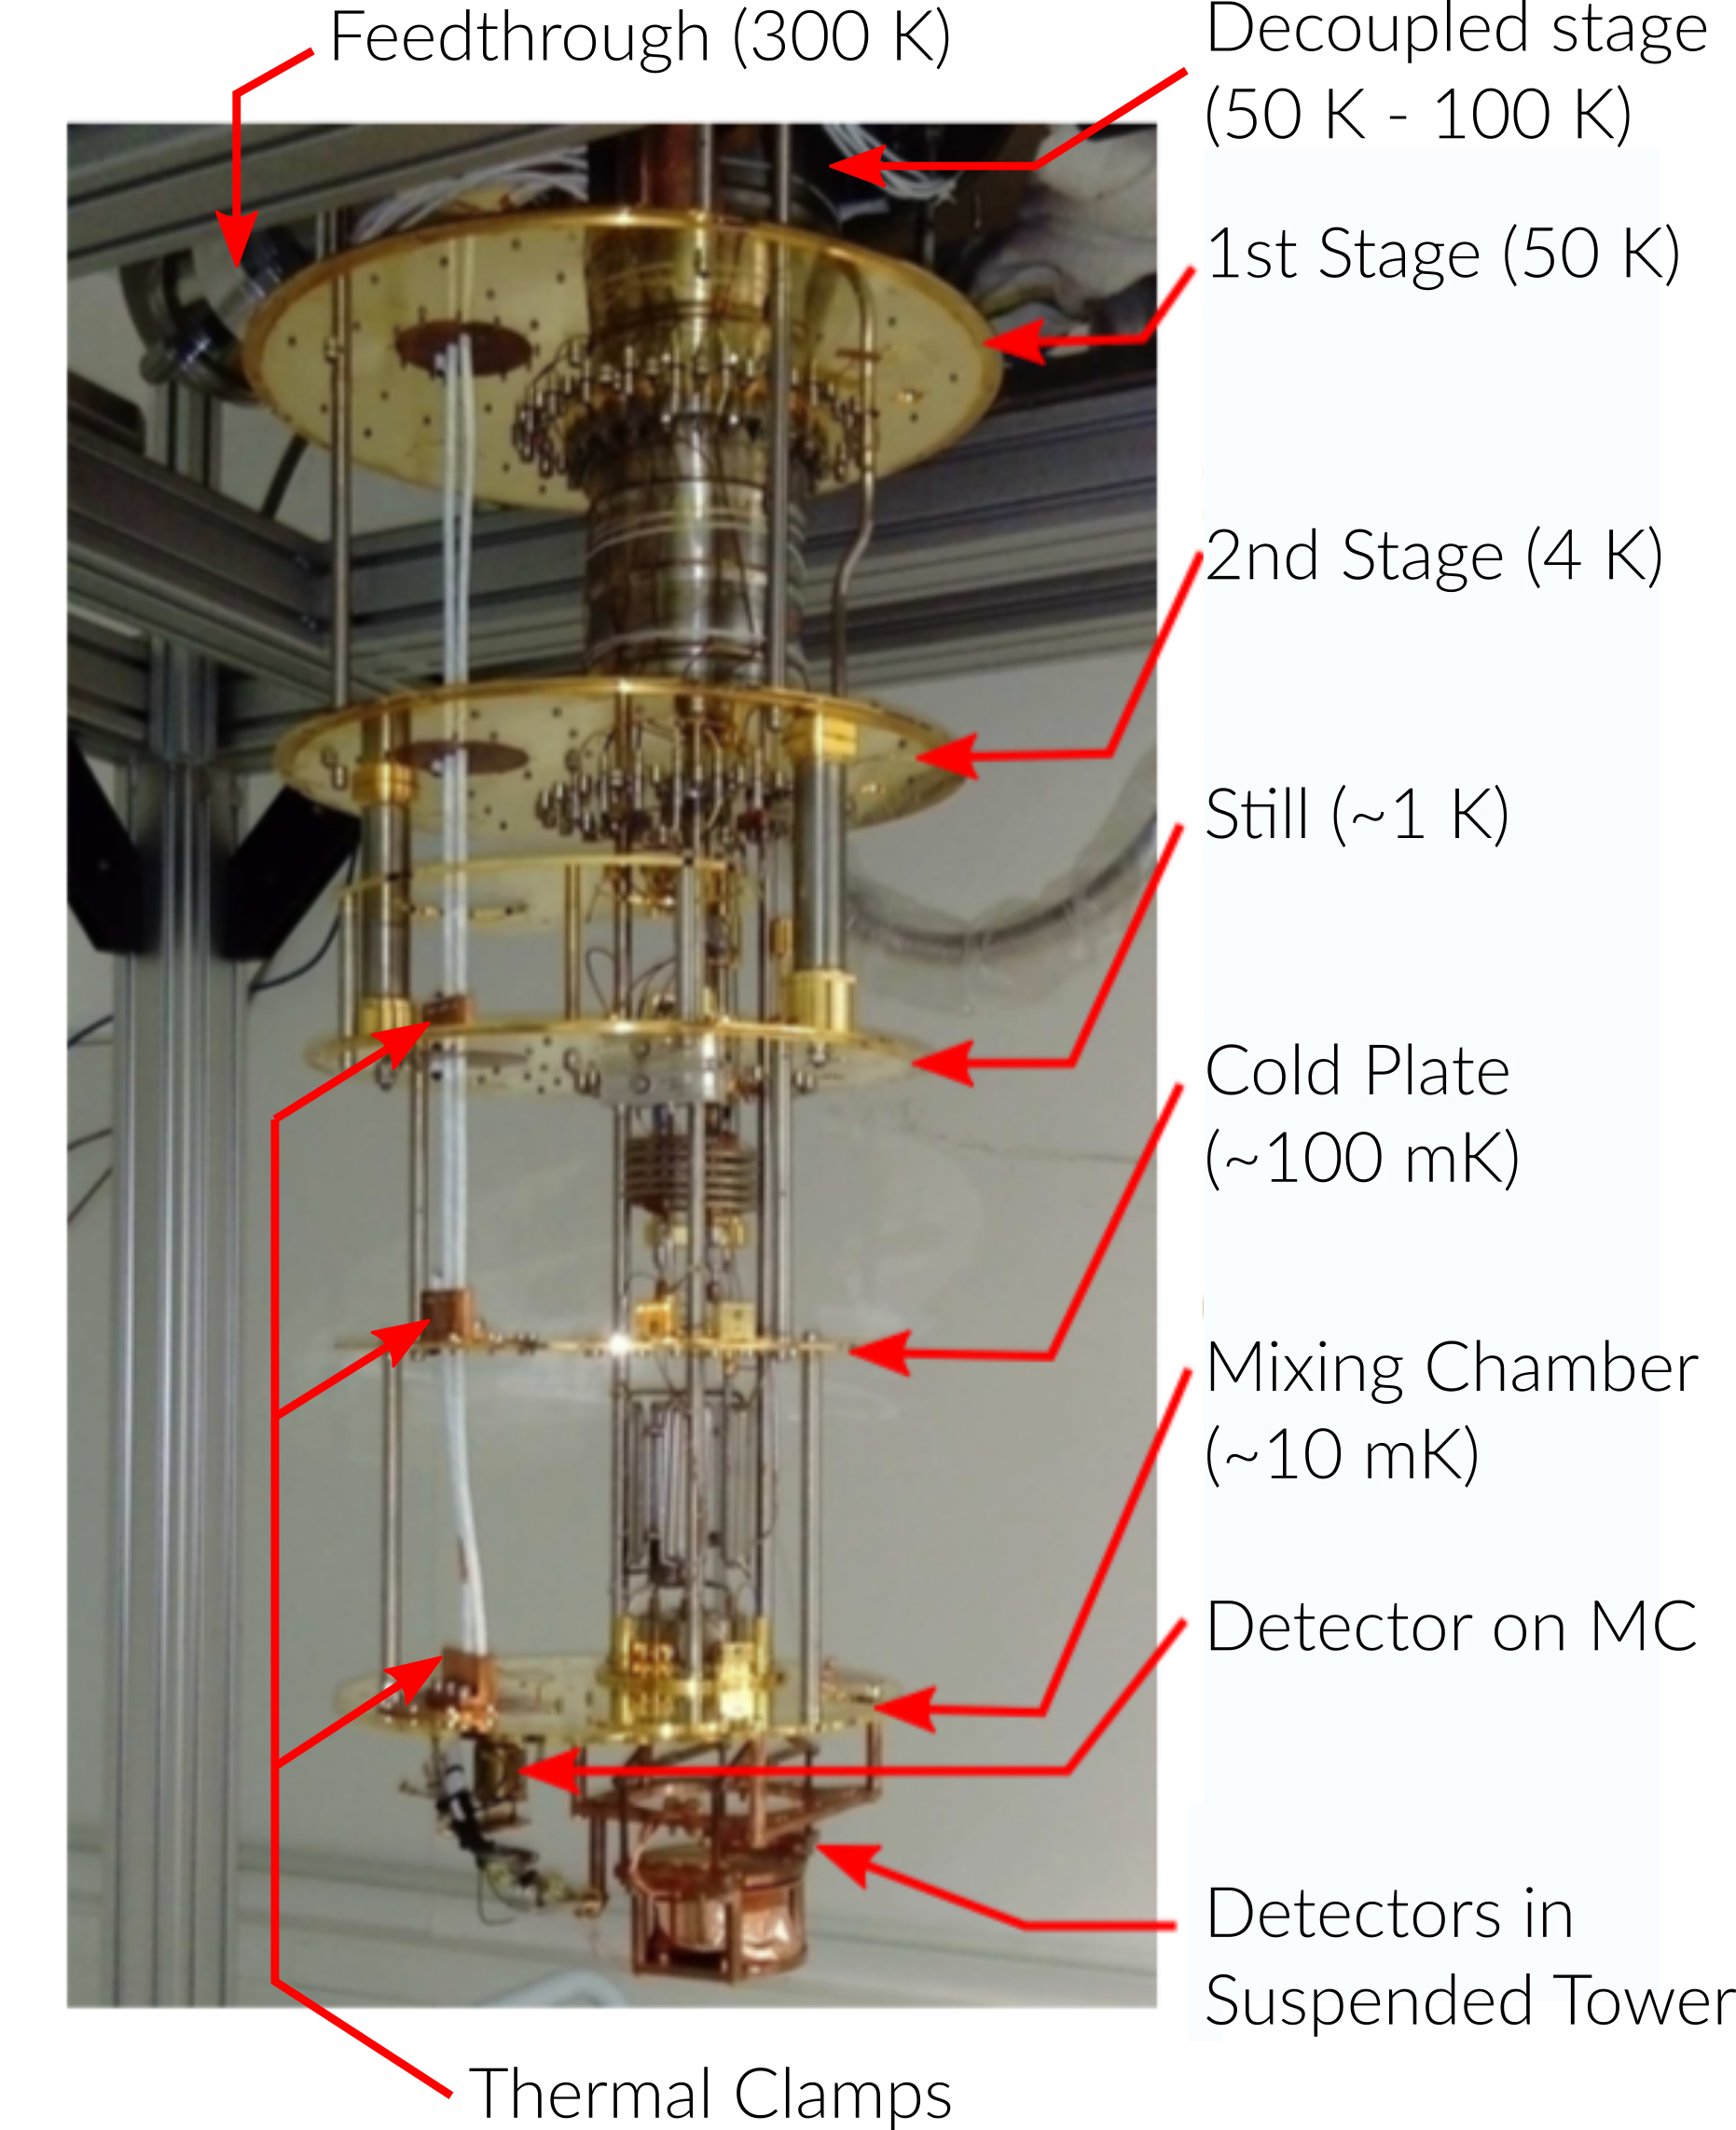
\includegraphics[width=\textwidth]{Figures/Experiment/cryo_photo.png}
\end{minipage}
\hfill
\begin{minipage}{0.48\textwidth}
	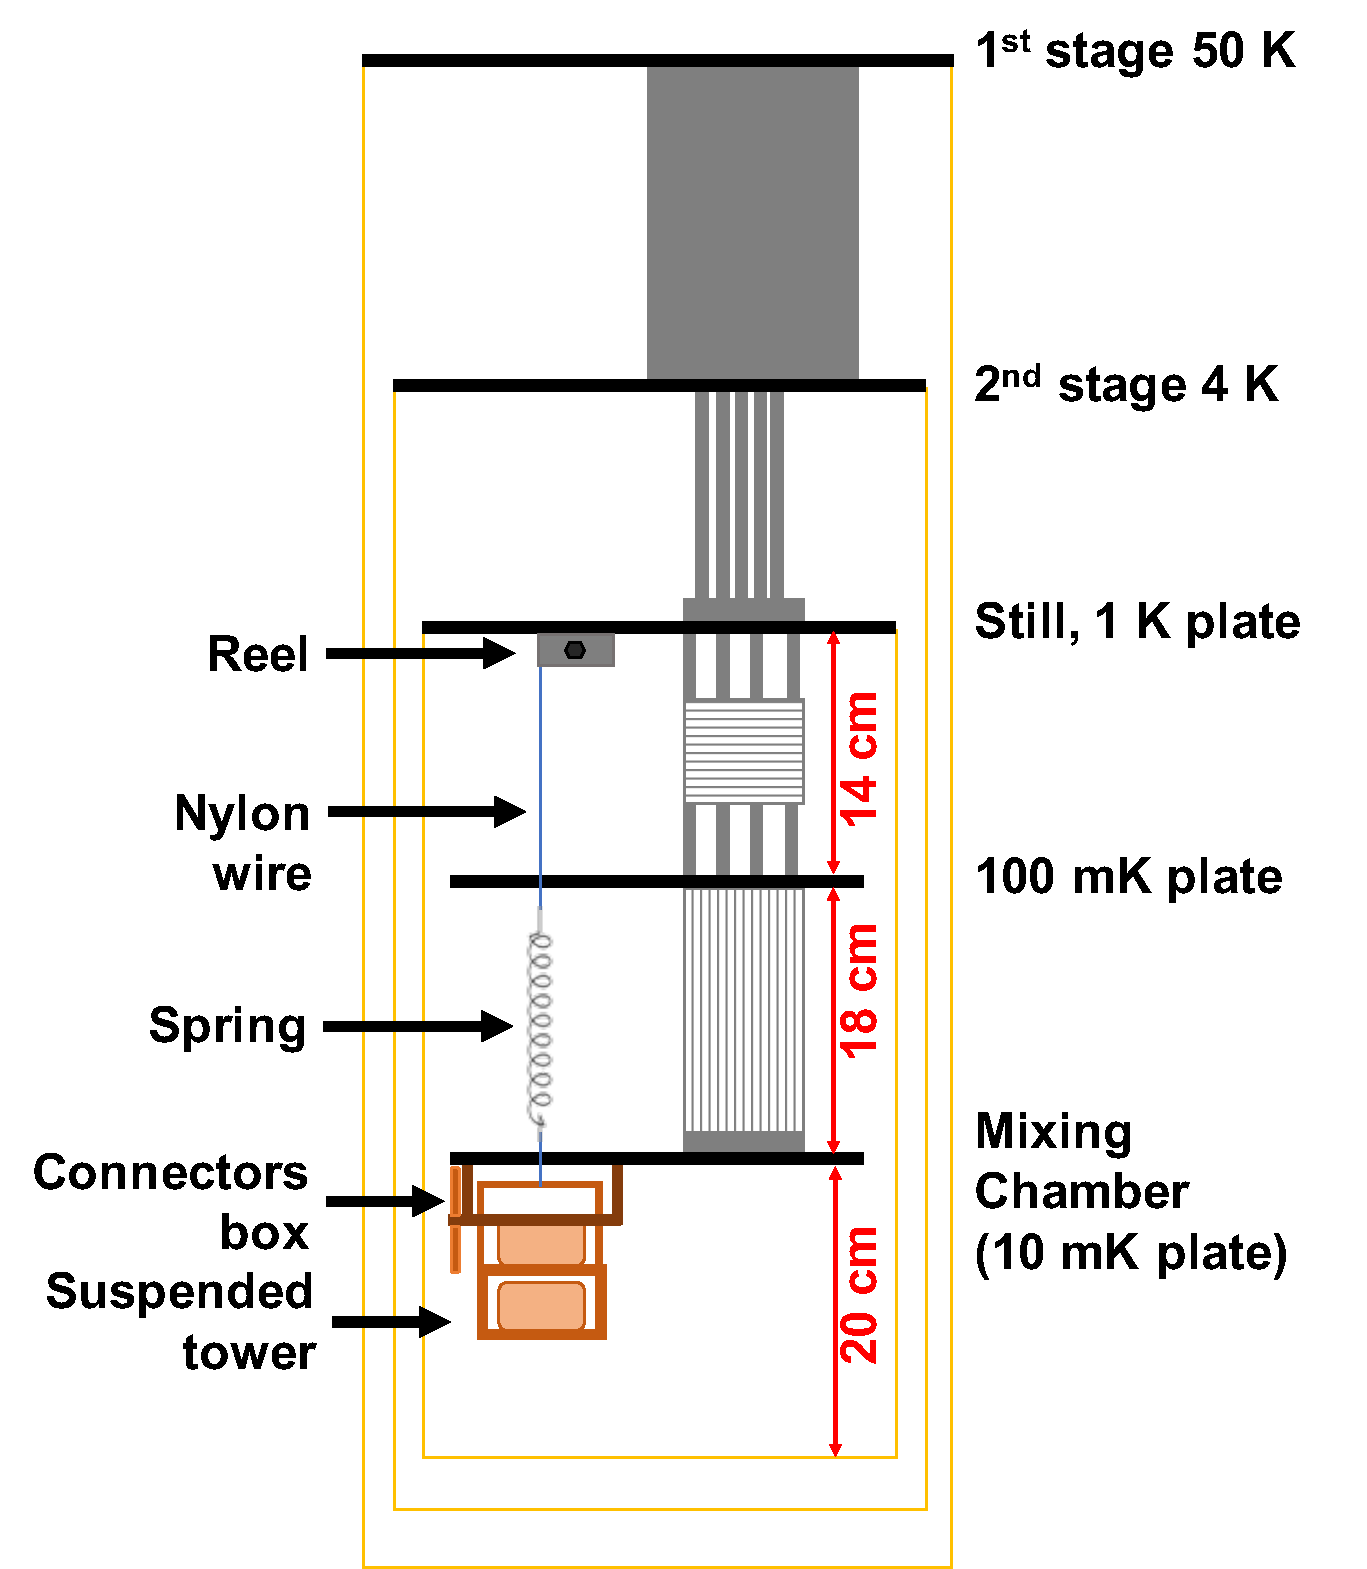
\includegraphics[width=\textwidth]{Figures/Experiment/cryo_sketch.pdf}
\end{minipage}
\caption{On the left, annotated photo of the open cryostat. On the right, annotated scheme of the cryostat. The copper screens blocking the infrared radiations are represented as the orange rectangles separating each cooling stage.}
\label{fig:cryo-photo} 
\end{figure}

% Dry cryostat
The IP2I cryostat is a Dry Dilution Refrigerators (DDR) the dry dilution cryogenic cooling technology. It runs solely on electric power as opposed to the Wet Dilution Refrigerators (WDR) of the EDELWEISS experiment which consumes liquid helium to cool down. Dry cryostats are particularly adapted to R\&D work as the operating cost are low and it is possible to descend very quickly to cryogenic temperatures (24 hours to reach \SI{4}{\kelvin}, compared to one week for the EDLWEISS cryostat at the LSM). They provides a similar low temperature environment as the one obtained with WDR at the cost of increased vibration levels. The IP2I cryostat was equipped with vibration mitigation solutions described in the next section \ref{sec:suspended-tower}.

% Cooling circuit
The IP2I dry cryostat has one closed cooling circuit using as cooling fluid a mixture of \ce{^4He} and \SI{25}{\percent} \ce{^3He}. This cooling circuit is separated in two cycles: the "Pulse Tube" cycle and the dilution cycle. 
% Pulse tube cycle
The pulse tube cycle is in charge of cooling the first stage and second stage to reach the temperatures \SI{50}{\kelvin} and \SI{4}{\kelvin} respectively. The "Pulse Tube" applies Stirling cycles between 9 and 18 bars at a frequency of \SI{1.6}{\Hz}, which allows the \ce{{}^4He} fluid to reach a temperature of \SI{4}{\milli\kelvin}.
% The dilution cycle
The dilution cycle extends the cooling circuit to the three other stages and cools them to their operating temperatures: the still at \SI{1}{\kelvin}, the cold plate at $\sim \SI{100}{\milli\kelvin}$ and the mixing chamber (MC) at $\sim \SI{10}{\milli\kelvin}$. In this cycle, the helium mixture is cooled by passing through fine capillaries located on the first and second stages, benefiting from the cooling of the pulse tube cycle. As the cooling fluid reaches \SI{4}{\milli\kelvin}, it condensates in its liquid phase. A succession of Joule-Thompson expansion valves and heat exchangers allows the mixture to reach a temperature of \SI{800}{\milli\kelvin} at the still. It is near this temperature that a phase separation occurs within the mixture: the first phase is concentrated in \ce{{}^3He} and floats on the surface of the second phase diluted in \ce{{}^3He} and rich in \ce{{}^4He}. This phenomenon can be explained by the Fermi-Dirac statistic followed by the \ce{{}^3He} atoms: they cannot simultaneously occupy the same energy state and the same position. Thus, for a sufficiently low temperature, the phase separation becomes energetically favorable. This phase separation takes place within the mixing chamber. The phase with low \ce{{}^3He} is then pumped out. The thermodynamic equilibrium of the two phases is broken and there is a transfer of \ce{{}^3He} from the concentrated phase to the diluted phase in \ce{{}^3He}. This process is endothermic, which decreases the temperature of the mixture and thus of the mixing chamber. The pumped helium \ce{{}^3He} is then re-injected into the dilution circuit. In this end, the dilution cycle allows a minimum temperature of \SI{9}{\milli\kelvin} to be reached on the mixing chamber for this cryostat. The detector load thermally linked to the mixing chamber in order to reach the lowest temperatures and the best performances.

% Thermal regulation
Once the cryostat is cooled down, it continues to operate at full power until the end of the run. The power of the cooling circuit is in constant equilibrium with the thermal heat coming from the exterior of the cryostat or from the operation of the detectors. Consequently, in this state, the exact temperature of the mixing chamber would fluctuates near its minimal equilibrium value. 
As a mean to operate the cryogenic detectors with constant performances at a chosen temperature order to stabilize, the temperature of the mixing chamber is regulated at higher temperatures usually superior to \SI{14}{\milli\kelvin}. The regulation is assured by the Joule effect of heating resistor. Its heat power is set by a Proportional-Integrate-Derivative controller (PID controller) reading the temperature with an \ce{RuO_2} thermistance close to the detectors suspended tower to choose exactly their operating temperature.


% detector load and electronics
We want to operate the bolometers at the coldest temperature possible. We may want to attach the detectors directly on the mixing chamber stage as seen on left photo of figure \ref{fig:cryo-photo}. However, the "dry" cryostat creates a lot of mechanical vibration especially due to the pulse tube cycle. These vibrations propagate to the detectors, causing thermal noise (parasitic phonons), electric noise (triboelectricity) as well as heat power on the mixing chamber which prevents a good cooldown.
% cite{Olivieri:2017lqz}
To tackle this issue, the cryostat is mechanically decoupled from the ceiling/pulse tube with a bellow (external decoupling). This external decoupling was done in partnership with Cryoconcept by mechanically decoupling the cold head of the pulse tube cryocooler from the dilution unit. The vibrations at the detector level were further mitigated by placing the bolometers inside a suspended tower (internal decoupling) developed by the Manoir group.
%\cite{romain}
The suspended tower is a copper chassis solely linked to the cryostat by a spring providing mechanical support and mechanical decoupling. This device makes it possible to avoid a significant low-frequency noise on the heat measurement while ensuring thermal conduction to the cryostat thanks to thin copper braids. This suspended tower is described in the paragraph \ref{sec:suspended-tower}.
% \cite{Maisonobe:2018tbq}

The detectors are cabled to the acquisition computer on the outside of the cryostat through the cold and warm electronics. The cold electronics function is transport the voltage signal of the detectors located near the mixing chamber to a first Bi-FET preamplifier stage at 100 K and a second stage amplifier at 300 K.
% ~\cite{Armengaud:2017rzu}
The white cables of this cold electronic are visible on the left photo of figure \ref{fig:cryo-photo}. The cabling comes from the top of the cryostat and goes down thermalizing at each stage with the thermal clamps. As such, only there is only minimal heat transfer from the hotter stages  on the mixing chamber due to the electronics.
Once the signal is amplified, it is transported to the acquisition computer with optic fiber. The detector signals are recorded as continuous time series called data streams. These data streams are then processed with a dedicated pipeline based on the NEPAL software developed by the Manoir group in order to ensure high quality data processing. The stream processing and analysis is described in the chapter \ref{ChapterElectrodesExperimental}. Once the processing is done at the CC-IN2P3, monitoring plots are transferred automatically to a monitoring website allowing us to follow the performance and behavior of the detectors as a function of time.

%%% Bonus
%% IP2I Cryostat for Ricochet 
%By early 2021, our cryogenic lab will be hosting the \Ricochet{} cryostat for a little over one year in order to be fully commissioned prior to its deployment at ILL. The commissioning phase includes: validation of the cabling (noise and thermal performance), the cold front-end electronics, the cool down of the inner shielding layers (lead and polyethylene), the demonstration of the CryoCube detector array performance (threshold, particle identification capability and livetime), and the DAQ and monitoring pipelines.


\section{Vibration mitigation and cryogenic suspension}
\label{sec:suspended-tower}

% Motivation
The cool-down process of the two first stages within DDR is ensured by the technology of pulse-tube cryocoolers. However, the mechanical vibrations they induce can drastically affect the performance of cryogenic detectors. This effect has been reported by several cryogenic experiments using such bolometers.
%\cite{Caparrelli:2006zkj,Haan:2013iwa,Olivieri:2017lqz}. 

% external mitigation
The IP2I cryostat was upgraded with an external vibration mitigation solution. Its first two stages (50K and 4K) are thermally coupled to the highly vibrating pulse-tube cold head thanks to low-pressure gas exchangers (Hexagas$^{\rm TM}$), hence avoiding any mechanical contact and vibration propagation to the dilution unit. In 2016, one year after its delivery to IP2I, the cold head has been mechanically anchored to the ceiling hence providing two independent and maximally decoupled frames. In the figure \ref{fig:cryolab}, the metallic framework surrounding the cryostat supports and anchors the dilution unit to the ground, while the cold-head is fixed in the ceiling of the laboratory (hidden by a wooden panel on the photo).

% results
This upgrade lead to the reduction of the vibration levels by about two orders of magnitude between \SI{0.5}{\Hz} and \SI{20}{\Hz} hence achieving world-leading vibration levels in a dry cryostat of few-\si{\micro g \per \sqrthz}.
 %below 20-Hz~\cite{Olivieri:2017lqz}.
At the time, the impact on our detectors has been tremendous. Indeed, before the decoupling, due to the high vibration levels, the detectors were not able to operate due to the significant vibration-induced  frictional heat power dissipation. 

% Motivation internal
% External Mitigation results 
With the improvement of our detector sensitivity and resolution, we found that the cold-head decoupling was not enough to ensure optimal operation of the new generation of detectors. Indeed, it was found that the large radial stiffness of the edge-welded below connecting the cold-head to the dilution unit still allows for some vibration propagation down to the detectors. A second vibration mitigation system at the mixing chamber level, where the detectors are installed, had to be implemented.


\subsection{Internal Mitigation Solution: the Suspended Tower}

%% Internal mitigation
%This internal vibration mitigation is the suspended tower presented in the annotated photo \ref{fig:suspended-tower}. This device consists in a 25 cm long elastic pendulum, attached to the \SI{1}{\kelvin} stage by a Kevlar string and a stainless steel spring with an elastic constant of \SI{240}{\newton\per\meter}, holding the detector tower situated below the mixing chamber at \SI{10}{\milli\kelvin}. The detector tower is thermally anchored to an intermediate safety structure via supple copper braids. This safety structure also hosts the connectors for the detector readout.

% suspended tower theory
This internal vibration mitigation solution is the suspended tower. A detector placed in this device can be considered mechanically as a simple elastic pendulum.
The 3-D dynamical description of the elastic-pendulum can be divided into two pseudo-independent equations in the approximation of small perturbations. The natural frequency for vertical modes is then given by:
\begin{equation}
f_{0,\textrm{vertical}}=\frac{1}{2\pi}\cdot\sqrt{\frac{k}{M}} = \frac{1}{2\pi}\cdot\sqrt{\frac{g}{(l_{\textrm{eq}}-l_{0})}}\label{eq:Freq-Vertical},
\end{equation}
where $M$ corresponds to the total mass of the suspended tower, $k$, $l_0$, and $l_{\rm eq}$ are the elastic constant, the rest length, and the length at equilibrium of the spring, respectively. The vertical resonance frequency can either be expressed of $k$ and $M$ simultaneously or by its elongation length alone $|l_{\textrm{eq}}-l_{0}|$. The natural frequency for radial oscillations of the pendulum, which are related to its total length  $l_{\rm tot}$, is given by:
\begin{equation}
f_{0,\textrm{ radial}}=\frac{1}{2\pi}\cdot\sqrt{\frac{g}{l_{\rm tot}}}\label{eq:Freq-Radial}.
\end{equation}
From these approximations, we can estimate the theoretical resonance frequencies of the elastic pendulum depending on the spring constant, the pendulum length and the total mass of the detector assembly. Interestingly, one can notice that as $l_{\textrm{tot}} \geq (l_{\textrm{eq}}-l_{0})$, the natural frequency in the radial direction is necessarily lower than in the vertical direction: $f_{0,\textrm{ radial}}<f_{0,\textrm{vertical}}$. 

Thanks to the use of a single spring holding system, we avoid any transverse momentum related natural frequencies which could populate the vibration spectrum at high frequencies. Therefore, system is expected to have a transfer function response under the form of a 2\textsuperscript{nd} order low-pass filter with a single resonance frequency in both directions $i=\left\{ \textrm{vertical, radial}\right\}$:
\begin{equation}
H(\omega_{i})=\frac{\omega_{0,i}^{2}}{\omega_{0,i}^{2}-\omega_{i}^{2}}\label{eq:Transfer-function},
\end{equation}
where $\omega_{0,i}$ is the natural pulsation of the suspended tower, with $\omega_{0,i}=2\pi\cdot f_{0,i}$. 
The natural frequencies of the suspended tower in both vertical and radial directions have been tuned to be as low as possible in order to attenuate all vibrations above \SI{1.4}{\Hz}, corresponding to the frequency of the pulse-tube cryocooler. According to equation \ref{eq:Freq-Vertical}, we obtain a vertical resonance frequency $f_{0,\textrm{vertical}} \leq \SI{1}{\Hz}$ for a spring elongation of at least $(l_{\textrm{eq}}-l_{0})\geq \SI{25}{\cm}$. The same condition applied to the radial frequency, $f_{0,\textrm{radial}} \leq \SI{1}{\Hz}$ results in a total pendulum length of at least  $l_{tot}\geq \SI{25}{\cm}$ using equation \ref{eq:Freq-Radial}.

The challenge then comes from accommodating with the constraints imposed by the cryostat geometry. As the distance between the mixing chamber plate and the inner thermal screen is only of about \SI{20}{\cm}, the pendulum had to be attached to the still plate and not directly to the mixing chamber.
The scheme of the figure \ref{fig:cryo-photo} and the photo \ref{fig:suspended-tower} illustrate the holding strategy of the suspended tower in the cryostat. 
A Kevlar wire is fixed below the still plate at \SI{1}{\kelvin} and running without contact through the cold plate at \SI{100}{\milli\kelvin}. 
A stainless steel spring with an elastic constant of $k=\SI{240}{\newton\per\meter}$ is attached to the wire between the cold plate and the MC at \SI{10}{\milli\kelvin}. The elastic constant $k$ has to be carefully chosen, taking into account the total mass of the detector assembly $M$, as its elongation is constrained by the $\sim \SI{18}{\cm}$ distance between the \SI{100}{\milli\kelvin} stage and the MC. 
Finally, the suspended tower is connected to the spring via a thick ($\sim \SI{2}{\mm}$ in diameter) \SI{5}{\cm} long copper wire through the MC plate. This copper wire ensures the thermalization of the stainless steel spring. so that it does not emit infrared radiation damaging the detector performance.
With this approach, the total pendulum length from the still plate to the center of mass of the detector assembly is $l_{\textrm{tot}} = \SI{25}{\cm}$.


\begin{figure}
\centering
\captionsetup{justification=centering}
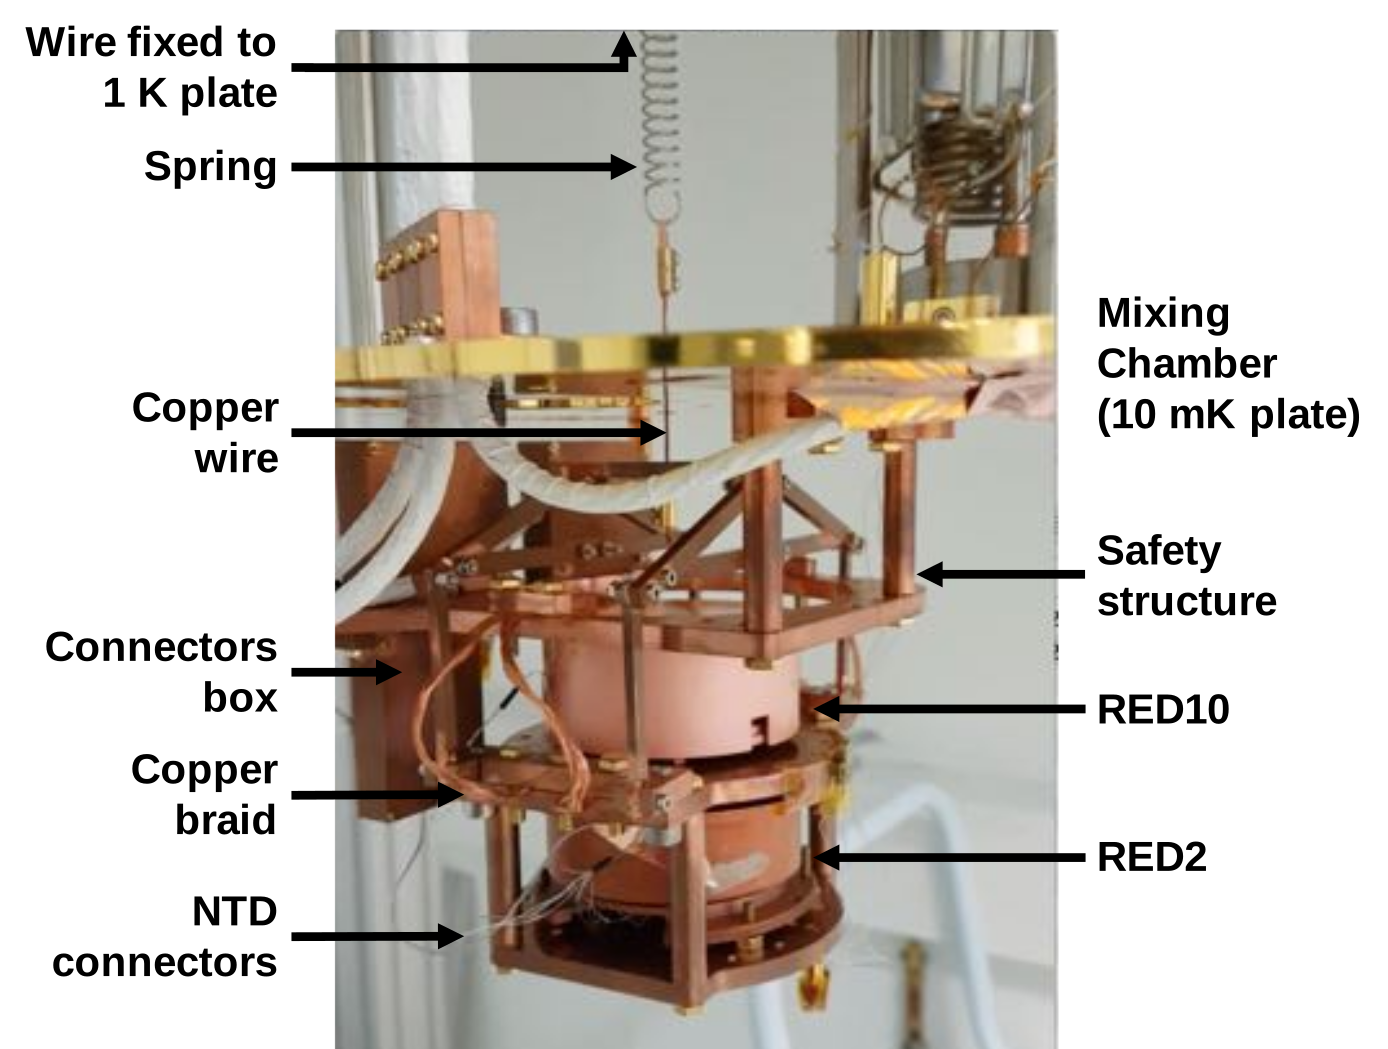
\includegraphics[height=9cm]{graphics/damocles.png}
\caption{Photo of the suspended tower containing the two $\SI{200}{\g}$ bolometers RED10 and RED2. This device mechanically decouples the detector load from the mixing chamber while assuring its thermalization.}
\label{fig:suspended-tower} 
\end{figure}

The detector tower is shown in the right panel of Fig\ref{fig:suspended-tower} holding the two detectors RED2 and RED10 . This module has a total height of \SI{13}{\cm} and can hold two cryogenic detectors based on \SI{200}{\g} germanium crystal or lighter. During the installation, before attaching the spring, the tower is firmly held by a copper frame screwed under the MC plate. This structure remains as a safety structure during cool-down and operation in case the wire should break. Connector boxes are placed close to the detector on the external side of the safety structure. They are used to connect the sensors of the detectors to the readout electronics at the warmer stages. Both the suspended tower and the safety structure are made of clean \ce{CuC_2} copper. During operation, the suspended tower is floating and its thermalization is realized by four \SI{10}{\cm} long ultra-supple flat copper braids linking the safety structure and the tower.


\subsection{Characterization of the Vibration Levels}

This subsection quickly presents the impact of the suspended tower on the vibration level and the noise of the heat channel of the bolometer RED10. All the results are published in the paper \cite{Maisonobe:2018tbq} in which the suspended tower was demonstrated to attenuate the transmission of both vertical and radial vibration, with a particular emphasis on the radial modes as these are less efficiently damped from our pulse-tube cold head decoupling. 

The vibration level is characterized by measuring the movement of the detectors.
%\cite{Olivieri:2017lqz}
The set-up is composed of a high sensitivity seismic accelerometer from \emph{PCB Piezotronics}. We used the high sensitivity accelerometer \emph{PCB-393B05} which has a gain of \SI{10}{\volt\per g} and an intrinsic noise limit of $\textrm{[0.5-0.07]}\,\textrm{g}/\sqrt{\textrm{Hz}}$ within $\textrm{[1-1000]}\,\si{\Hz}$ frequency range.

The accelerometer is fixed on U-shaped workpiece allowing to measure the vibrations along either the radial or the vertical direction.  The accelerometer can be fixed below the MC stage of the cryostat, or below the bottom stage of the suspended tower in order to compare their respective vibration level. 
The elastic constant $k$ and Young's modulus $E$ values of the stainless steel and copper, composing the majority of the rigid strucutre of the cryostat, have small variation between ambient and cryogenic temperature. As such, all vibration measurements are performed at room temperature.
%~\cite{Emodulus}.
The output signal of the accelerometer is sampled at \SI{10}{\kilo\Hz}, well beyond the signal bandwidth of the accelerometer of \SI{1}{\kilo\Hz}. The vibration levels is obtained as LPSD expressed in \si{g \per \sqrthz} from a Fast Fourier Transform (FFT) analysis using Hanning windowing over \SI{5}{\s} time windows.
Figure~\ref{fig:Status-Tower-vibrations-PTonoff} displays the vibration levels on the MC plate and in the suspended tower comparing the measurements with the pulse-tube (PT) cryocooler switched on (PT ON), emulating the normal cryostat operation, or off (PT OFF). The intrinsic noise limit of the accelerometer is plotted as dashed lines as reference.

\begin{figure}
\centering 
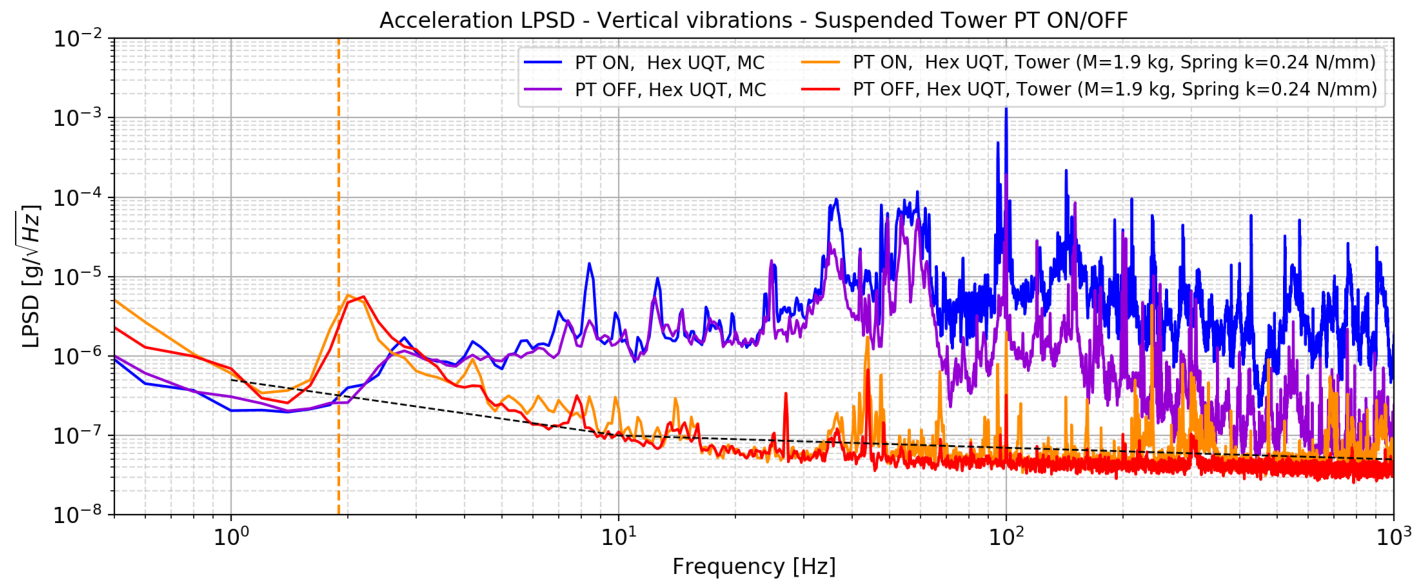
\includegraphics[width=\textwidth]{Figures/Experiment/vibration_vertical.pdf}
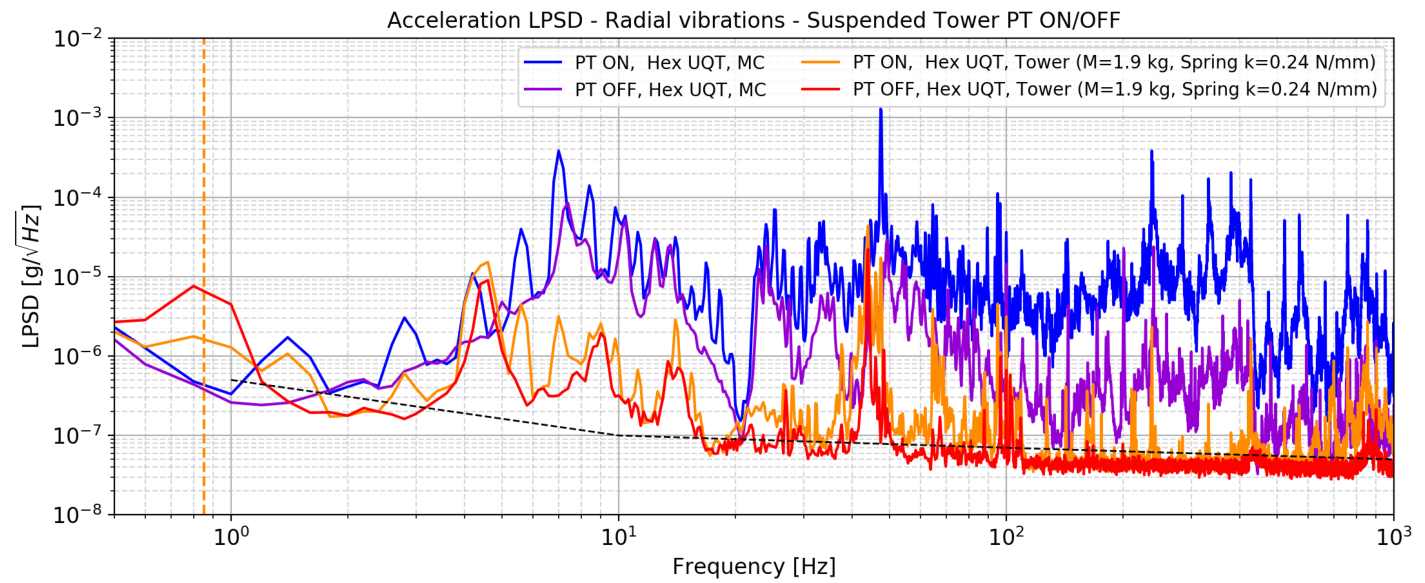
\includegraphics[width=\textwidth]{Figures/Experiment/vibration_radial.pdf}
\caption{Comparison of the vertical (top subplot) and radial (bottom subplot) vibration levels of the MC plate and the suspended tower in both PT ON and OFF configurations. The dashed black line is the accelerometer sensitivity, and the orange vertical dashed lines represent the position of the natural frequencies of the suspended tower derived from equations \ref{eq:Freq-Vertical} and \ref{eq:Freq-Radial}.}
\label{fig:vibration-levels}
\end{figure}
%  Figures taken from~\cite{Maisonobe:2018tbq}.

The main differences observed between these two PT configurations are coming from few pick-up lines which are mostly at high frequencies and arise from the acoustic noise generating by the operation of the pulse-tube cooling cycle.
At low frequencies ($<\SI{40}{\Hz}$), in the detector bandwidth, the impact of turning the PT ON is very small on the suspended tower, merely being expressed as resonance peaks of low amplitude.
As a matter of fact, by comparing the vibration level of the MC plate at PT OFF case (purple solid line) to the level of the suspended tower at PT ON case (orange solid line), one can further conclude that the suspended tower is not only efficient at reducing the PT-induced noises but also most of the whole setup-related vibrations from the building, the cryostat holding structure, and so on.
this demonstrate that vibration-wise, our detectors are largely insensitive to their surrounding environment, suggesting that they should run in optimal conditions inside the IP2I cryostat.

% Noise level for RED10
This optimal operations condition can be check by comparing the noise level affecting the signal measurement of a detector either installed on the mixing chamber plate or in the suspended tower. In this paragraph, this comparison is made with the \SI{200}{\g} detector RED10 whose heat channel is later characterized in the chapter \ref{ChapterEthem}. With a heat sensitivity of about \SI{100}{\nano\volt\per\kilo\eV} at around \SI{18}{\milli\kelvin}, RED10 is sensitive to perturbative displacements and vibrations. 

The noise levels are presented as LPSD expressed in \si{\volt\per\sqrthz}. These LPSD were measured as presented in the paragraph \ref{par:ethem-noise} dedicated to the characterization of the electronics noise affecting the heat channel of the bolometers.

Figurec \ref{fig:red10-vibration} shows the LPSDs obtained for RED10 on the MC plate as dashed lines, and on the suspended tower as solid lines. The \SI{1}{\volt} normalized heat signal template power spectrum and the theoretical noise calculations based on the full electro-thermal modeling of the detectors (see Sec.~\ref{sec:ethem-noise}) are also plotted as references. Measurements of the LPSDs were made with and without polarizing the NTD of RED10 in order to estimate the effect of the vibrations on the cabling, such as microphonics. Note that the discussion will mostly focus on the frequency range of interest, from \SI{1}{\Hz} to \SI{40}{\Hz}, as it corresponds to the detector signal bandwidth.

\begin{figure}
\centering 
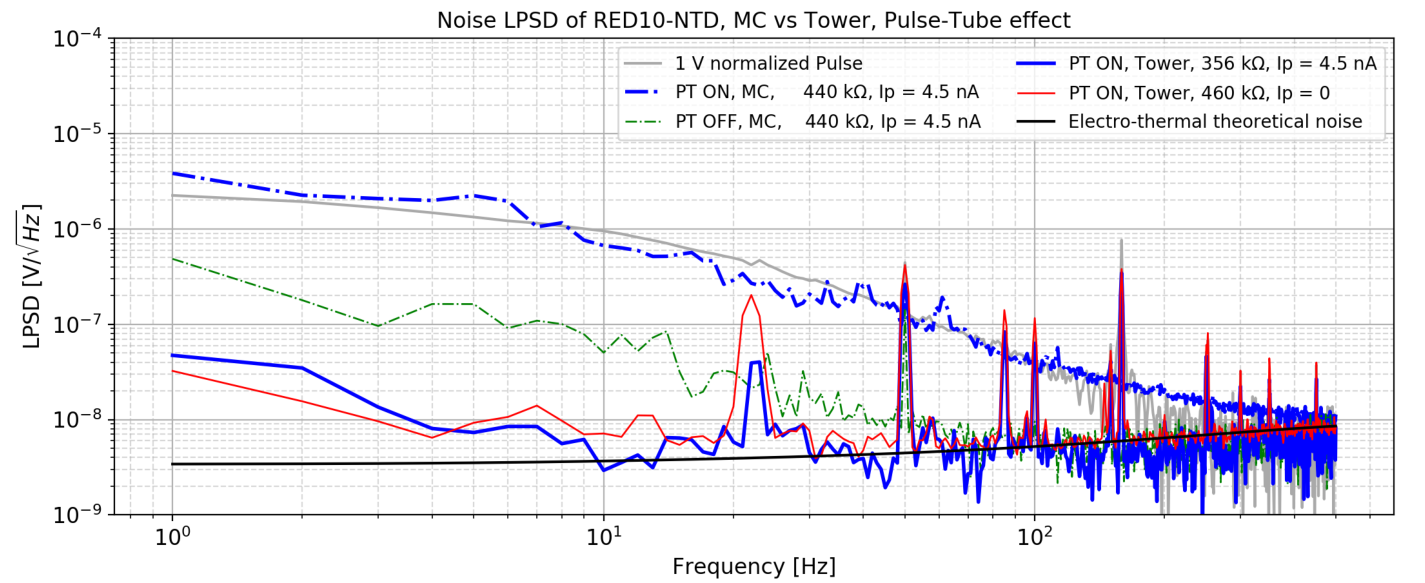
\includegraphics[width=\textwidth]{Figures/Experiment/red10_lspd_vibration.pdf}
\caption{Noise power spectra density for the NTD of RED10 mounted on the MC plate (dashed lines) and on the suspended tower (solid lines). Measurements were performed at optimal NTD polarization currents with PT ON and PT OFF at \SI{16}{\milli\kelvin}. The black solid line refers to the expected noise level derived from the electro-thermal model described in section \ref{sec:ethem-noise}, while the grey solid line shows the unit normalized pulse template illustrating the signal bandwidth.}
% Figures taken from~\cite{Maisonobe:2018tbq}.
\label{fig:red10-vibration}
\end{figure}


From comparing the various voltage PSD presented in Figure~\ref{fig:Noise-LPSD-RED2}, we can extract a few major conclusions regarding the effectiveness of the suspended tower at mitigating the vibration-induced noise on bolometers. 

The first obvious comparison is between the cases where the detectors are optimally polarized (blue curves) and either on the mixing chamber (dashed lines) or on the suspended tower (solid lines). The LPSD at the lowest frequencies is reduced by almost two orders of magnitude. 
Furthermore, we observe that the noise levels obtained PT ON and with the NTD optimally polarized (blue solid lines) are almost identical to the case where the NTDs are not polarized and the pulse-tube OFF (red dashed lines), suggesting that we are limited by both the electronics and the intrinsic thermal noise from the detector, and not by the vibrations when the detectors are mounted on the tower.
 This is confirmed by the fact that the resulting noise levels are very close to the theoretical expectations obtained with the electro-thermal model illustrated by the black solid lines.

Interestingly, we do not see on any of the three NTDs a \SI{1.8}{\Hz} pick-up noise as was potentially suggested from the vertical acceleration measurements shown as the red (PT OFF) and orange (PT ON) solid lines from Figure~\ref{fig:vibration-levels}. This  suggests that such frequency vibrations within the detector bandwidth do not limit the detector performance.

Finally, one can derive from Figure~\ref{fig:red10-vibration} that the noise PSD obtained with the NTDs optimally polarized on the suspended tower with PT ON (blue solid lines) are below the ones obtained with the detectors running on the mixing chamber with the PT OFF (green dashed lines). This observation confirm what was suggested from the vibration measurements shown in figure \ref{fig:red10-vibration}:  the suspended tower damps very efficiently the vibration-induced noise from the pulse-tube cryocooler, but makes the detectors insensitive to any residual vibrations from the surrounding environment of the experiment

The improvement on RED10 performances can be appreciated by computing its energy resolution. It was found that the heat resolution RED10 from \SI{14}{\kilo\eV} when installed on the mixing chamber, to \SI{400}{\eV}  when installed in the suspended tower. This impressive gain of almost two order of magnitude on the energy resolution can be explained by the detector RED10 being especially susceptible to vibrations. This detector would have been discarded due to poor performances without this internal mitigation solution.

%\footnote{Note that since this work, tremendous progress have been made on the low-noise cold cabling, the processing tools, and the low-energy calibration, such that RED10 actually achieved 50~eV (RMS) heat energy resolution later on, see Sec.~\ref{sec:randd-heatperformance}}.

Following the publication of this work~\cite{Maisonobe:2018tbq} similar improvement factors were found, between a factor of a few up to one order of magnitude, on all of the detector prototypes of the RED series.
The detectors operated at in the iP2I cryostats are no longer limited by vibrations, but only by the intrinsic JFET-based electronic noise limiting us from reaching the ultimate thermal fluctuation noise floor.
Based on this success, a new suspended tower
%shown in Fig.~\ref{fig:newtower}
that can host up to 5 RED detectors was installed in the IP2I cryostat in early 2020.  Though a similar elastic pendulum approach would not be feasible in the \Ricochet{} cryostat for the CryoCube, a slightly different three-spring pendulum approach is currently being investigated  for optimal operation of the CryoCube detector  at ILL.

%%% Bonus
%% Other mitigation solutions
%Several approaches have been considered to mitigate vibrations in dry dilution refrigerators: CUORICINO~\cite{DAddabbo:2017efe, Pirro:2006mu}, CUORE and its 988 TeO$_2$ detector array~\cite{Ligi:2016ldu,Santone:2017tjm}, and more recently the LUMINEU and CUPID-Mo collaborations with their three springs detector towers each hosting three to four crystals in the EDELWEISS cryostat in Modane~\cite{Armengaud:2017hit}. The CUORE experiment has implemented a different strategy. A Y-Beam (with three connecting points) at 300~K, isolated from the cryostat through \emph{Minus-K} suspensions, supports the whole 988 TeO2 detector array. Despite the use of three CRYOMECH PT415 pulse tubes, they report keV-scale detector energy resolutions \cite{Ligi:2016ldu,Santone:2017tjm}. Other implementations of passive decoupling systems on DDR, with a large panel of physics applications, can be found in \cite{Pelliccione:2012wx,Haan:2013iwa}.

%\cite{Olivieri:2017lqz}
%This suspended tower design reduces detector vibrations at the sub-$\mu$g/$\sqrt{\text{Hz}}$ level, with displacements in the order of a few nanometers (RMS) in all three axes, leading to substantial gains in energy resolutions
%as demonstrated in Ref.~\cite{Maisonobe:2018tbq}. 


%----------------------------------------------------------------------------------------
%	PRINCIPLES BOLOMETERS
%----------------------------------------------------------------------------------------
\section{Principle of Cryogenic Bolometers}

all of the bolometers discussed hereafter were fabricated by our collaborators at IJCLab, CEA Saclay, and Institut N\'eel.

 It is also equipped with a system of cameras in order to monitor the gluing process, usually performed with AW106 epoxy


\begin{figure}[!ht]
\begin{minipage}{0.45\textwidth}
\includegraphics [width=\textwidth]{Figures/Experiment/red10_photo_annotated.pdf}
\end{minipage}
\caption{(left) Photograph of the R\&D cryostat of the Manoir team at the IPNL. The detector in the suspended tower is RED10. The Dyonisos detector is a detector studying the ionization pathway, it is not studied in this report. \\ (right) Annotated photograph of the RED10 detector.}
\label{photo}
\end{figure}

In both experiment, we are searching for an interaction between a particle (WIMP or neutrino) and a nucleus (see fig \ref{cenns-process}). What is interesting us is the measurement of the energy of this process we call a nuclear recoil. 

\begin{figure}
\centering
\captionsetup{justification=centering}
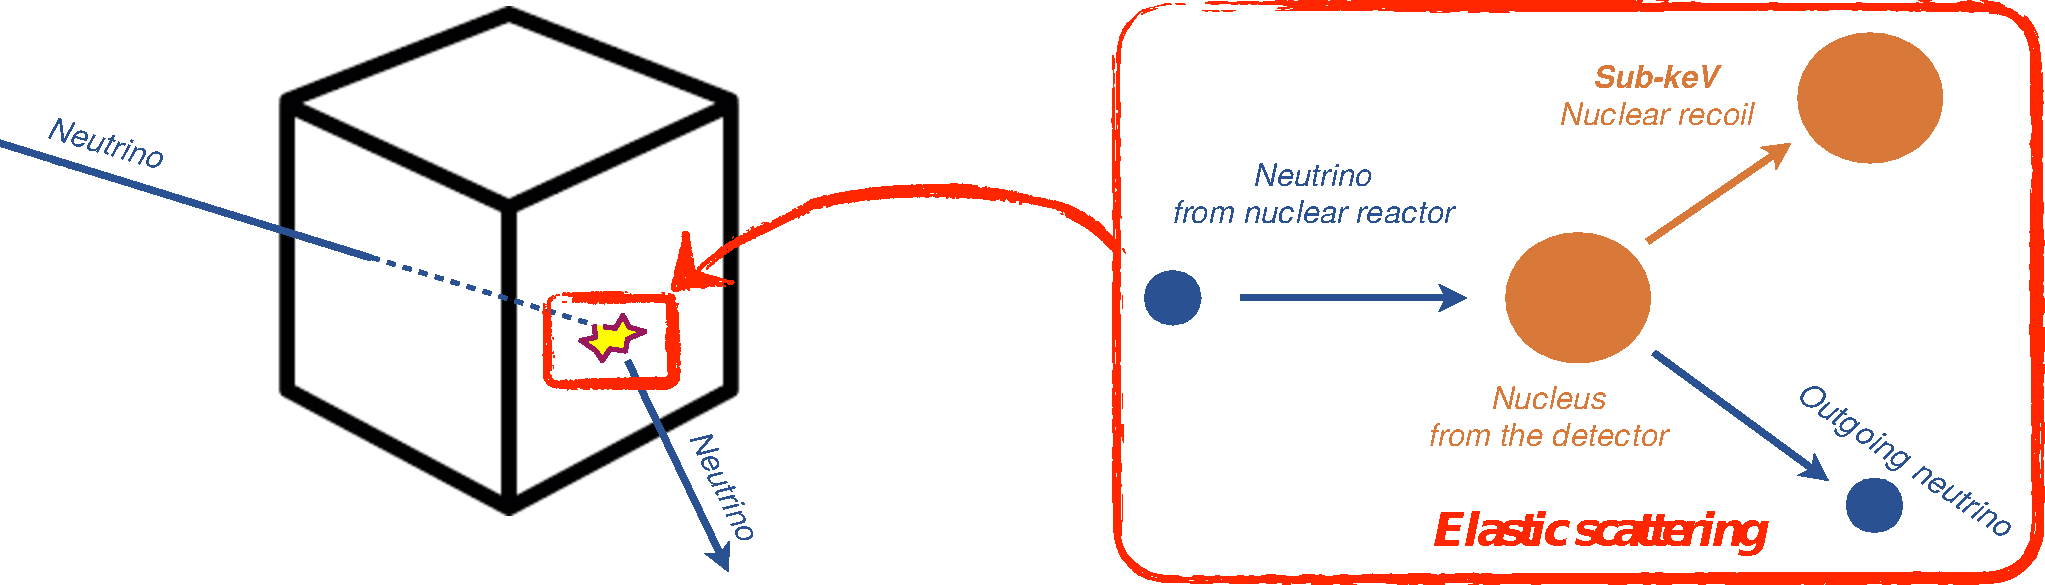
\includegraphics[width=\textwidth]{Figures/Experiment/cenns_process.pdf}
\caption{\label{cenns-process} \em Scheme of the CENNS process. The cube represents the absorber of a bolometer. This process is similar to a nuclear recoil caused by a WIMP-nucleon interaction (mentally replace neutrino/nucleus by WIMP/nucleon and you got the associated scheme)}
\end{figure}

This nuclear recoil energy can be expressed in several ways, depending on the target material: production of light, production of phonons or production of electron-holes pairs (ionization). For this lab work, the studied detectors are composed of semiconducting germanium crystal. The energy deposited by a nuclear recoil $E_R$ will produces phonons and ionization. Produces phonons will eventually thermalize and increase the temperature of the germanium crystal. A very sensitive thermometer can pick up this thermal signal $\Delta T$ (in Kelvin) while several electrodes applying an electric field in the crystal will collect the electrons and holes and register an ionization signal $\Delta V$ (in Volt). In an ideal system, the energy conservation gives:

\begin{equation}
\label{energy}
E_R = E_{ph} + E_{e-h}
\end{equation}

with the thermal energy $E_{ph}$ depending on the thermal capacity of germanium crystal $C_{Ge}$ (in $J.K^{-1}$):

\begin{equation}
E_{ph} = C_{Ge} \times \Delta T
\end{equation}

and the ionization energy $E_{e-h}$ written as:

\begin{equation}
E_{e-h} = n_{e-h} \times \epsilon_{Ge} = \frac{C_{el} \times \Delta V}{q_{e}} \times \epsilon_{Ge}
\end{equation}

with $n_{e-h}$ the number of electron-holes pairs, $\epsilon_{Ge}$ the energy of an electron-hole pair ($\approx 3$ eV in Ge), $C_{el}$ the electric capacity of the electrodes and $q_{e}$ the elementary charge. The ratio between phonon and ionization energy is the same for every nuclear recoil of a given energy such that we can introduce a quenching factor $\epsilon = f(E_R)$ such that:

\begin{equation}
\label{quenching}
E_{e-h} = \epsilon \times E_R \quad \textsf{and} \quad E_{ph} =(1-\epsilon) \times E_R
\end{equation}

\begin{figure}
\centering
\captionsetup{justification=centering}
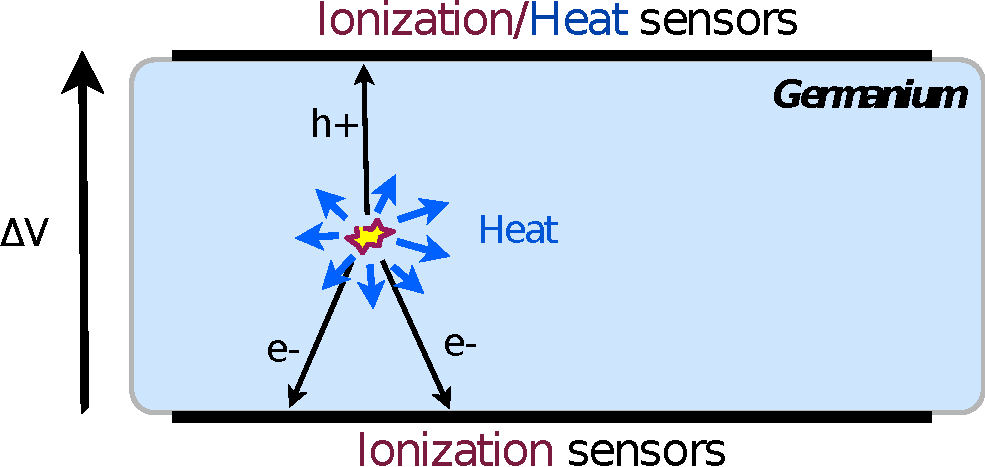
\includegraphics[width=0.7\textwidth]{Figures/Experiment/ge_detector.pdf}
\caption{\label{ge-principle} \em Scheme of the measurement channels in a germanium bolometer.}
\end{figure}

This kind of detector is called a bolometer as it is measuring the heat (heat channel) to estimate the nuclear recoil energy (see eq \ref{quenching}). Measuring the charges in the crystal (ionization channel) gives a second estimate of this energy thus allowing some discrimination between good event (nuclear recoil) and parasitic events ({\em e.g.} electron recoil from natural radioactivity). In order to work with semiconducting germanium (which is essential for the ionization channel), the temperature of the crystal must be low enough. Additionally, the heat channel becomes sensitive enough at the lowest temperatures which are only achievable in a cryostat.
This double-measurement design in a cryogenic bolometer (sum up in fig \ref{ge-principle}) is a characteristic of the EDELWEISS experiment and will be in use for RICOCHET. Most of the other dark matter and CENNS experiments have chosen different strategies (light channel, single measurements channel, Luke Neganov boost, other target material, etc..).

\section{Studied Cryogenic Bolometers: RED50 \& RED60}

For this lab work, you are studying one of the two new bolometers from the "RED" series, RED50 and RED60 (see fig \ref{bolo-photo}), which were assembled and installed in the cryostat a few days ago. The RED series are R\&D-focused bolometers aiming at a full understanding and optimization of the heat and ionization channel. The new bolometers RED50 and RED60 are 32g crystal germanium upon which is glued a single Neutron-Doped Transmuted (NTD) germanium thermistor (see fig \ref{bolo-photo}). The resistance $R$ of the NTD depends on its temperature $T$ following the equation \ref{ntd-law} where $R_0$ and $T_0$ are the characteristic resistance and temperature for the NTD.

\begin{equation}
\label{ntd-law}
R(T) = R_0 \exp \left( \sqrt{ \frac{T_0}{T} } \right)
\end{equation}

Several gold wires link the NTD electrodes to the cabling (elevated gold pads on photo) on the copper chassis, thus assuring electric and thermal conduction. The germanium crystal is maintained with Teflon pads and sapphire balls inside the copper chassis. An Fe55 source is fixed inside the copper chassis facing the germanium crystal, it is use for calibration purpose (Gamma at 6keV).

Contrary to the usual EDELWEISS detectors, RED50 and RED60 do not possess electrodes and were assembled for the study of the heat channel. The electron-holes pairs created by a nuclear recoil simply recombine because of the lack of electric field. This recombination process produces additional phonons in the crystal. This means that the ionization energy $E_{e-h}$ is converted into thermal energy $E_{th}$, and equation \ref{energy} simply becomes $E_R = E_{th}$.



\subsection{Functioning of RED1 and RED10 detectors}

In order to obtain very low energy thresholds on the detectors used, and to meet the $4\times $100 objective, it is essential to understand the response of the detectors as well as possible. In particular, the recently launched heat path optimization campaign requires the construction of a thermal model of the detectors. These models and optimization designs are tested and validated with experimental measurements in the R\&D cryostat of the Manoir group.

These studies are carried out within the framework of the EDELWEISS collaboration with the RED detector series (Research and Development). This series of detectors focuses on heat channel measurements: these detectors have a very pure design allowing to test thermal models and to better understand the physical processes involved in the detector. 

In this report, two detectors are used and studied: RED1 and RED10. A picture of the RED10 detector is presented in the figure (\ref{photo}). The design of these two detectors is extremely similar, their difference is based on the NTD geometry and the type of glue used. First of all, an ultra-pure semiconductor germanium crystal acts as an absorber: it is the element that serves as a target for the elastic collision of the WIMPs, thus recovering the recoil energy expressed as phonons and ionization. This makes it possible to have a material with very heavy cores ($Z=74$), which improves the exposure to the WIMPs flow, while having a low thermal capacity $C$ (evolving like the cube of temperature). Thus, the recoil energy $E$ expressed as heat will cause the absorber temperature $T$ to vary according to the formula :
\begin{equation}
\Delta T = \frac{E}{C}
\label{capa}
\end{equation}
The germanium crystal is held by teflon fasteners to the copper support to prevent thermal conduction with the cryostat.

A neutron-doped germanium thermistor called NTD (Neutron Transmutation Doped) is bonded to this absorber. As its electrical resistance depends very strongly on its temperature, it acts as a thermal sensor.  Surfaces and gold wires ensure a thermal leakage to the copper support at the constant temperature of the cryostat. The NTD thermistor is connected to a polarization and acquisition circuit. The resistance of an NTD follows the law of Efros and Shllovskii \cite{mccammon}:

\begin{equation}
\label{eq:ntd-resistivity}
R_{NTD}(T) = R_0 \cdot \exp(\sqrt{\frac{T_0}{T}})
\end{equation}

where $R_0$ and $T_0$ are a characteristic resistance and temperature of the NTD used. They depend on the geometry of the NTD, its doping, and the external constraints applied to it. In the case of RED1, we have $R_0=1.04 \Omega$ and $T_0=4.77 \textrm{K}$. Although this thermistor is made of germanium, it is doped and its physical properties are changed: it is conductive and thus has a free electron system in addition to a phonon system. The phonon system has a thermal capacity evolving like the cube of the temperature as the absorber (low thermal capacity), while the capacity of the electron system is linear with the temperature (high thermal capacity). We can therefore understand the usefulness of having an absorber-sensor couple: one serves as a target for the deposition of energy with low thermal capacity, while the other allows the measurement of the temperature rise. Cryogenic temperatures are necessary to be in a temperature range where the NTD thermistor becomes sufficiently sensitive to temperature variations.

It is necessary to build a model of the complete detector in order to characterize the response to a WIMP event and the noise on the measurement. This will allow to evaluate the energy resolution of the detector and to study the influence of the different parameters on it.

%This chapter describes the work done during the last four months in a Manor group. It first explains the development of an electro-thermal model to simulate a detector. This is followed by a description of the analysis used to characterize the electronics from experimental data obtained with the RED1 detector already characterized. Then is presented the characterization of a new RED10 detector based on the constructed model and new experimental measurements. Finally, the comparison between the resolutions of the experiment and the simulation allows to verify the validity of the model and to define the next research tracks.


\subsection{Detector}
\label{sec:detector}

The detector prototype, called RED20, is shown in Fig~\ref{fig:EDWdetector}. It consists of a cylindrical high-purity Ge crystal of 20 mm diameter and 20 mm height, corresponding to a total mass of 33.4-g. 
The thermal sensor design has been optimized for enhanced heat energy resolution. It consists of a Ge-NTD of $2\times 2\times 0.5$ mm$^3$, glued on the top surface of the crystal, weakly thermally coupled to the copper housing of the detector thanks to gold wire bonds connecting its electrodes to two gold pads on a Kapton tape.   
With a total Ge-NTD electrode surface of 2 mm$^2$ this weak thermal link is about 2.1~nW/K which is sub-dominant with respect to the electron-phonon coupling of 6.7~nW/K ensuring that the detector properly integrates all of the heat signal~\cite{Pyle:2015pya}.

The crystal is held by six PTFE clamps (three on each side) in order to ensure the mechanical constraints on all three axes of displacement and to minimize the stress due to PTFE elasticity at low temperatures. Unlike the usual EDELWEISS-III FID800 detectors~\cite{Armengaud:2017rzu}, this detector prototype has only one heat channel and no ionization readout. Therefore, a discrimination between nuclear and electron recoils is not possible. However, as there is no electric field applied across the crystal, the detector acts as a true calorimeter measuring the deposited energy of the recoiling particle independently of its type (nuclear or electronic recoil).
Quenching effects on the heat energy scale for nuclear recoils in Ge cryogenic detectors have been shown to be very small~\cite{Benoit:2006qc,Agnese:2018nbs}, and are therefore neglected hereafter. 


\section{Calibration Sources}

- Muons of high energy
The detector RED10 was then calibrated using the $\sim \SI{18}{\mega\eV}$ muon peak. 

- Iron 56 source at 6keV
An $^{55}$Fe calibration source was glued on the inner part of the detector's copper housing and facing the crystal surface opposite to the side on which is glued the Ge-NTD.

- KLM lines of activated germanium


% From jules colas

\section{Prototype detectors}

Members of the RICOCHET collaboration at IP2I are working on prototypes similar to the future elements of the CRYOCUBE detector. These prototype detectors form the series detectors called RED. While all the RED detectors possesses a heat measurement channel only some are equipped with electrodes for the ionization measurement channel. 


\subsection{Heat measurement}

The NTD-Ge, which allows the measurement of temperature variations of the germanium crystal, works like a thermistor whose resistivity decreases as the temperature rises. It is polarized, i.e., a direct current $I$ of a few \si{\nano\ampere} is applied to give a representation of the resistance in tension from Ohm's law $V = R \cdot I$. The value  of the resistance of an NTD-Ge evolves according to the relation
\begin{equation}
\label{eq:ntd-resistivity}
R_{NTD}(T) = R_0 \cdot \exp(\sqrt{\frac{T_0}{T}})
\end{equation}
with $R_0$ and $T_0$ constants specific to each sensor. The temperature measurement allows to estimate the energy deposition thanks to the thermodynamic relation:
\begin{equation}
\Delta T = \frac{\Delta E}{C_{th}}
\end{equation}
where $C_{th}$ is the thermal capacity of the detector. The exponential relation allows to obtain a large variation of voltage for a small temperature variation. In RED detectors, an energy deposit $\Delta E \sim \si{\kilo\eV}$ induces a temperature variation of the order of \si{\micro\kelvin} and leads to tensions measured from a few hundred \si{\nano\volt}. The detectors are kept at low temperature by a thermal link with the cryostat characterized by a heat conductance $G$. This link results in an exponential thermalization of the detector with a time constant $\tau \sim C_{th}/G$. In practice, the heat signal is modeled by decaying exponential pulses with several characteristics times associated with the different thermalization processes and calorific capacities.


\subsection{Ionization measurement}

The measurement of electron-hole pairs created during the deposition of energy by an incident particle is done by collecting charges on electrodes. These are made by evaporating a metal on the surface of the target material. An electrical voltage is then imposed between them, the electric field induced in the material will then allow to accelerate the charges up to the electrodes. We can note the variation of voltage $\Delta V$ read at the terminals of the electrodes as a function of the collected electrical charge $\Delta Q$ and the electric capacitance of the electrode $C$: 
\begin{equation}
\Delta V = \frac{\Delta Q}{C}
\end{equation}
Compared to a heat pulse, the charge collection process is very fast. As much so that the signal $\Delta V$ is modeled by a Heaviside function translated by $t_0$ the instant
interaction of a particle in the crystal:
\begin{equation}
\begin{cases}
\forall t < t_0, \Theta(t - t_0 ) = 0 \\
\forall t \leq t_0, \Theta(t - t_0 ) = \Delta V
\end{cases}
\end{equation}



%%% FRom Julien HDR


Crystalline cryogenic detectors (bolometers) aim at measuring the heat signals, in the form of thermal or athermal phonons, induced by a particle interaction following $\Delta T = E_r/C$ where $\Delta T$ is the corresponding temperature increase and $C$ the heat capacity of the system (see Fig.~\ref{fig::dets}~b). Cryogenic detectors are operated in the 10-to-50~mK range to minimize the heat capacity and the thermal fluctuation noise. Several temperature sensing techniques exist, but the most widely and mature ones are the (low-impedance) Transition Edge Sensors (TES) and neutron transmutation dopped germanium (NTD-Ge) thermistors. In both cases, the heat increase is measured via a change in resistance which is either measured as a current or voltage drop at the front-end of the readout electronics. A wide variety of crystal materials can be used, but in recent years the leading materials have been: CaWO$_4$ in CRESST~\cite{Abdelhameed:2019hmk}, Ge and Si in (Super)CDMS~\cite{Agnese:2013ixa}, and Ge in EDELWEISS~\cite{Armengaud:2017rzu}. Interestingly, a simultaneous measurement of a second observable, such as ionisation in semiconductors (Ge, Si) or scintillation in scintillating crystals (CaWO$_4$), allows for electronic/nuclear recoil discrimination as in both cases the ionization/scintillation yields vary with the recoiling particle type. Cryogenic detectors feature a precise energy measurement with almost no quenching in the heat channel, excellent energy resolution and background rejection down to energies of $\mathcal{O}$(1)~keVnr. The operation at mK-temperatures is challenging and expensive. Additionally, the requirement of a low-energy threshold constrains the mass of the individual detectors, limiting the reachable exposure. Cryogenic experiments have therefore progressively focused their efforts in searching for light DM candidates, usually below 10~GeV, as threshold then becomes more important than exposure.\\



\section{Searching for low-mass dark matter with EDELWEISS}
\label{sec:EDELWEISS}

The EDELWEISS experiment has been initiated in the 90's and has completed  its third phase, operated from the {\it Laboratoire Souterrain de Modane} (LSM), the deepest European's laboratory. With an overburden of about 4800~m.w.e the muon flux at LSM has been measured to be of 5~muons/m$^2$/day~\cite{Armengaud:2017rzu}. Figure~\ref{fig:EDW-All-Simu-Text} (left panel) shows the technical drawing of the EDELWEISS setup at LSM. The dilution refrigerator hosting the bolometers is surrounded by 20~cm of lead (including 2~cm of roman lead), 50~cm of polyethylene, and a 100~m$^2$ active muon veto~\cite{Armengaud:2017rzu}. The reversed cryostat, allowing access to the bolometers from the top, can host up to 40~kg of cryogenic detectors in its 50~liter experimental volume. Based on previously acquired experience in the limiting surface backgrounds, the EDELWEISS-III experiment operated 24 FID800 cryogenic detectors. Figure~\ref{fig:EDW-All-Simu-Text} (right panel) shows a picture of a FID800 detector which are made of ultrapure germanium cylindrical crystals with a height of 4~cm, a diameter of 7~cm and a mass of 820-890~g~\cite{Armengaud:2017rzu}. These detectors are instrumented to perform a double heat-and-ionization measurement of signals arising from particle interactions. The double read-out is used to discriminate background-induced electron recoils (ER) from potential WIMP-induced nuclear recoils (NR) on an event-by-event basis. \\

Heat signals are measured with two Neutron Transmutation Doped (NTD) Ge sensors~\cite{Armengaud:2017rzu} glued at the center of the top and bottom surfaces of the crystal\footnote{It is worth noticing that the FID800 detectors also have a 20~mm$^2$ gold pad on the top surface used to tune the thermal leak. This is a major difference with the RED detector prototypes presented in Chap.~\ref{chap:CryoCube} and~\ref{chap:randd} where the thermal leak is done through the NTD itself.}. The resulting temperature dependence of NTD-Ge heat sensors is well described by the Shklovskii-Efr\"os law given by~\cite{Mathimalar:2014sfa}:
\begin{equation}
    \rho(T) = \rho_0\exp(\sqrt{T_0/T})
\end{equation}
where $\rho_0$ depends on the intrinsic properties of Ge and of geometrical factors, and $T_0$ is related to the germanium doping level. As exemplified by the previous equation, the NTD resistance increases quickly with lowering the temperature. They are usually tuned to have 1-100 M$\Omega$ resistance values in the 7-20 mK temperature range. The heat pre-amplification electronics in EDELWEISS-III is based on IFN860 bi-JFETs, allowing for a differential readout, with an AC modulated current in the 500 Hz range. This differential modulation technique has been originally developed for the Archeops balloon and Planck satellite to efficiently reject both the electronics $1/f$ contribution and common-mode noise sources~\cite{Armengaud:2017rzu}. 



Ionization signals are measured thanks to the 200~nm thick Al electrodes  evaporated on the whole Ge crystal, both flat and side surfaces, in the form of annular concentric rings 150~$\mu$m wide with a 2~mm pitch. The concentric electrodes are connected electrically such that all odd-numbered rings are connected to each other as well as all even-numbered rings. This leads to four groups of electrodes, {\it i.e.} 2 collecting and 2 surface veto electrodes, allowing an efficient discrimination between bulk and surface events. The FID800 electrode capacitance is about 100~pF and they are readout with a voltage pre-amplifier using IF1320-JFET. As further discussed in chapter~\ref{chap:CryoCube}, despite their low-noise application, the ionization resolution is limited from the intrinsic current noise from this JFET-based electronics.\\



The EDELWEISS and SuperCDMS experiments have pioneered the use of cryogenic semiconductor crystals (Ge and Si) to search for Dark Matter particles. Following a particle's interaction in the detector medium, the induced recoil (electronic or nuclear) will release its energy by creating both phonons (heat) and charge carriers (ionization). 
To first order\footnote{We neglect here the phonon energy loss due to Frenkel defects~\cite{Agnese:2018nbs, Benoit:2006qc} and to charge trapping}, the different measurable energy quantities are intertwined as follows:
\begin{align}
    E_{ion} & = Q(E_R) E_R \\
    E_{NTL} & = E_{\rm ion}\frac{V}{\epsilon} \\
    E_{heat} & = E_R + E_{\rm NTL} = E_R\left[1+Q(E_R)\frac{V}{\epsilon}\right]
    \label{eq:GeNTL}
\end{align}
where $V$ is the voltage bias and $\epsilon$ is the average energy required for an electron recoil to produce an electron-hole pair. $E_{heat}$ and $E_{ion}$ stand for the heat and ionization energies, respectively. $E_{NTL}$ is the additional Neganov-Trofimov-Luke heat energy produced by drifting the charge carriers across the crystal~\cite{Luke,Neganov:1985khw}. The quenching factor $Q(E_R)$ is equal to 1 for electronic interactions by definition, whereas it is between 0 and 0.3 for nuclear recoils between 0 and 20~keV~\cite{Barker:2013nua}. Following Eq.~(\ref{eq:GeNTL}), two operating modes can  be considered:

{\bf NR/ER discrimination mode:} By operating the detector at bias voltages low enough, such that $E_{NTL} \ll E_R$ for nuclear recoils, the simultaneous measurement of heat and ionization provides an event-by-event identification of the recoil type, hence allowing a highly efficient rejection of the dominant gamma backgrounds as well as the majority of beta-backgrounds. Residual gamma- and surface beta-backgrounds are further removed using the active surface rejection, thanks to veto electrodes, of the FID detector design~\cite{Armengaud:2017rzu}. It is worth highlighting  that, in addition to the event-by-event discrimination, the simultaneous heat and ionization energy measurements also provides a direct measurement of the true nuclear recoil energy, hence avoiding any assumptions on the ionization yield to be made. 

{\bf NTL boosted mode:} By operating the detector at high voltage biases ($\geq$ 100 V), the cryogenic calorimeter is effectively turned into a charge amplifier of mean gain $(1+Q(E_R)\frac{V}{\epsilon})$. As $E_{heat} \simeq E_{ion}$, event-by-event discrimination is no longer possible and an ionization yield model has to be assumed to convert the total heat energy into a nuclear recoil energy equivalent. It should be noted that, thanks to the much higher ionization yield of electron recoils compared to nuclear recoils, this operation mode is highly beneficial to any DM searches looking for interactions with the electrons instead of nuclei.  \\


The EDELWEISS collaboration successfully achieved an average baseline energy resolution (RMS) of 400~eV and 200~eVee for the heat and ionization channels, respectively. Thanks to the double heat and ionization measurement, EDELWEISS has demonstrated a gamma and surface-beta rejection factors better than $< 2.5 \times 10^{-6}$ and $< 4\times 10^{-5}$ at 90\% C.L. respectively, while keeping a nuclear recoil acceptance of about 75\% down to a nuclear recoil energy of 15 keV~\cite{Armengaud:2017rzu}. Thanks to these detector performance, the collaboration achieved leading exclusion limits on SI interactions for WIMP masses from 5 to 30 GeV/c$^2$~\cite{Hehn:2016nll} (purple limit in Fig.~\ref{fig:si_status}), provided the first measurement of the cosmogenic activation rate of tritium in Ge above-ground~\cite{Armengaud:2016aoz}, and derived leading limits on ALP dark matter candidates~\cite{Armengaud:2018cuy}. The next phase of the EDELWEISS experiment, called EDELWEISS-SubGeV, aims at probing DM particle candidates within the eV/$c^2$-to-GeV/$c^2$ mass range by considering both DM interactions on electrons and nuclei. 

In this context, the collaboration has recently demonstrated a 55 eV heat energy threshold on a 33.4 g Ge detector operated above ground leading to the most stringent above-ground limit on SI interactions above 600~MeV/c$^2$~\cite{Armengaud:2019kfj} (see Chap.~\ref{chap:Surf} and purple limit in Fig.~\ref{fig:si_status}). To enhance its sensitivity to DM particle masses from 500~MeV/c$^2$ to 5~GeV/c$^2$, and in synergy with \Ricochet{}, the collaboration is also developing new electrode designs and electronics to lower the particle discrimination threshold from $\sim$1~keV to 50~eV in low voltage mode~\cite{Juillard:2019njs}. Lastly, the collaboration recently achieved an impressive 6~eVee energy threshold with a 33.6~g Ge detector operated at LSM in a high voltage mode (78 V). Figure~\ref{fig:RED30} (left panel) shows the event energy distribution following a $^{71}$Ge activation where we can clearly identify the x-ray lines from the electron-capture decays from the K/L/M shells at 10.37~keV, 1.3~keV, and 160~eV respectively. Thanks to this exquisite energy resolution, the collaboration has achieved the first Ge-based sub-100~MeV/c$^2$ dark matter search and the most stringent limit on Dark Photons below $\sim 10$~eV/c$^2$~\cite{Arnaud:2020svb}, as shown in Figure~\ref{fig:RED30} (right panel). These first results are pathfinders to the upcoming EDELWEISS-SubGeV detector technology that will operate 30~g-scale Ge detectors both in low- and high-voltage modes for maximum sensitivity to various DM models. The CryoCube detector technology, currently being developed in the context of a precise measurement of the CENNS process at a nuclear reactor with \Ricochet{} (see Chap.~\ref{chap:ricochet} and ~\ref{chap:CryoCube}), is a good candidate for the low-voltage approach. The high-voltage approach is being investigated within the SELENDIS Marie-Curie fellowship program and its follow-up CryoSEL project.

\begin{figure}
\centering
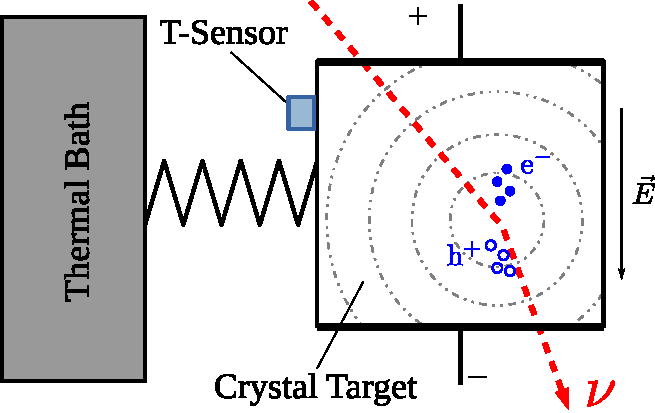
\includegraphics[scale=1]{Figures/Experiment/crystalline_detector_principle.pdf}
\caption{Working principle of crystalline bolometer (here with additional charge-readout) for particle detection. Images adapted from ~\cite{Schumann:2019eaa}}
\label{fig:crystalline}
\end{figure}



%----------------------------------------------------------------------------------------
%	BONUS UNUSED
%----------------------------------------------------------------------------------------

%\section{Detector principle}
%
%\begin{equation}
%\begin{cases}
%Q = Q_{ER} = 1 \\
%E_{Ion.}^{bulk} = Q \cdot E_R = E_R \\
%E_{heat} 
%=
%E_R 
%\cdot
%\frac{
%1 + Q_{ER}\frac{V_{bias}}{\epsilon_{e^--h^+}}
%}{
%1 + \frac{V_{bias}{\epsilon_{e^--h^+}}
%}
%= E_R
%\end{cases}
%\end{equation}
%
%\begin{equation}
%\begin{cases}
%Q = Q_{NR} \left( E_R \right) \\
%E_{Ion.}^{bulk} = Q_{NR}\left( E_R \right) \cdot E_R \\
%E_{heat} 
%=
%E_R 
%\cdot
%\frac{
%1 + Q_{NR} \left( E_R \right)\frac{V_{bias}}{\epsilon_{e^--h^+}}
%}{
%1 + \frac{V_{bias}{\epsilon_{e^--h^+}}
%}
%\end{cases}
%\end{equation}
%
%\begin{equation}
%\begin{cases}
%Q = Q_{HO} = 0 \\
%E_{Ion.}^{bulk} = Q_{NHO} \cdot E_R = 0 \\
%E_{heat} 
%=
%E_R 
%\cdot
%\frac{
%1 + Q_{HO} \left( E_R \right)\frac{V_{bias}}{\epsilon_{e^--h^+}}
%}{
%1 + \frac{V_{bias}{\epsilon_{e^--h^+}}
%}
%=
%E_R 
%\cdot
%\frac{
%1
%}{
%1 + \frac{V_{bias}{\epsilon_{e^--h^+}}
%}
%\end{cases}
%\end{equation}



%\section{Meaning of the stream name}
%
%Each recorded stream of data is denominated by a sequence of characters. This sequence depends on the date of the run and blah blah.
%
%TO DO Explanation.